% !TeX program = xelatex
% 编译：xelatex main.tex  连跑两遍
\documentclass[12pt,a4paper]{ctexart}

\usepackage[margin=2.5cm,top=2.8cm,bottom=2.5cm]{geometry}
\usepackage{graphicx}
\usepackage{booktabs}
\usepackage{array}
\usepackage{amsmath}
\usepackage{caption}
\usepackage{enumitem}
\usepackage[hidelinks,unicode]{hyperref}

\setCJKmainfont{SimSun}[BoldFont=SimHei, ItalicFont=KaiTi]
\setCJKsansfont{SimHei}
\setmainfont{Times New Roman}

\linespread{1.45}
\setlength{\parindent}{2em}
\captionsetup{font=small,labelsep=quad}
\setlist[itemize]{leftmargin=2em,itemsep=2pt,topsep=4pt}

\title{\vspace{-1.2cm}\textbf{面向低空物流的无人机感知界面设计}\\[4pt]
\large 从深度估计误差到风险可读性的一次人机交互实践}
\author{}
\date{}

\begin{document}

% ============ 封面 ============
\begin{titlepage}
\centering
\vspace*{2.2cm}

{\zihao{2}\bfseries 《小白学人工智能》课程论文}

\vspace{0.6cm}
{\zihao{4}（2026--2027 学年第一学期）}

\vspace{2.6cm}

{\zihao{2}\bfseries 面向低空物流的无人机感知界面设计}

\vspace{0.5cm}
{\zihao{4}从深度估计误差到风险可读性的一次人机交互实践}

\vspace{1.2cm}
{\zihao{4}＿＿＿＿＿，＿＿＿＿＿，＿＿＿＿＿}

\vspace{2.4cm}

{\zihao{4}
\renewcommand{\arraystretch}{1.9}
\begin{tabular}{rl@{\hspace{2.4cm}}rl}
课程名称 & 小白学人工智能 & 任课教师 & 李\quad 粤 \\[2pt]
学\qquad 院 & ＿＿＿＿＿＿＿ & 专业班级 & ＿＿＿＿＿＿＿ \\[2pt]
学生一 & ＿＿＿＿＿＿＿ & 学\qquad 号 & ＿＿＿＿＿＿＿ \\[2pt]
学生二 & ＿＿＿＿＿＿＿ & 学\qquad 号 & ＿＿＿＿＿＿＿ \\[2pt]
学生三 & ＿＿＿＿＿＿＿ & 学\qquad 号 & ＿＿＿＿＿＿＿ \\
\end{tabular}}

\vfill
{\zihao{5}2026 年 11 月}
\end{titlepage}

% ============ 摘要 ============
\begin{center}
{\zihao{3}\bfseries 面向低空物流的无人机感知界面设计}\\[4pt]
{\zihao{5}从深度估计误差到风险可读性的一次人机交互实践}
\end{center}

\vspace{0.4cm}

\noindent{\bfseries 摘\quad 要：}无人机在城市楼宇间配送时只有一枚摄像头，前后距离必须由算法估计，而算法会出错。更麻烦的是，它出错时地面看屏幕的人察觉不到，界面上只有一条飞行轨迹。

本文训练单目深度估计模型并测出其在仿真城市飞行数据上的准确度，其中 ImageNet 预训练骨干的验证集 $\delta_1$ 达到 0.86，但在玻璃幕墙与远景结构画面上仍会误判。针对这一失效模式，设计一套地面站界面：左栏机队列表按风险排序，中栏主视图提供三种信息密度的呈现模式，右栏把模型判断、测量值、置信度与操作分区陈列。测试让非专业被试在系统已触发悬停的场景下判断是否应当解除，记录判断正确率、反应时间，以及模型出错时被试是否跟着出错。

这套方案用于检验一个假设：界面若只复述模型结论，人会在模型出错时一起出错；保留可解读的中间信息，才能让人察觉异常。

\vspace{0.3cm}
\noindent{\bfseries 关键词：}人机交互；无人机；单目深度估计；界面设计；自动化偏见

\vspace{0.8cm}

\begin{center}
{\zihao{4}\bfseries Design of a Perception Interface for Low-Altitude\\
Logistics Drones}\\[4pt]
{\zihao{5}From Depth Estimation Error to Risk Readability}
\end{center}

\vspace{0.3cm}

\noindent{\bfseries Abstract:} A delivery drone threading through urban canyons carries a single camera, so range must be inferred by an algorithm, and the algorithm errs. Worse, when it errs the person watching the screen cannot tell, because the interface shows only a flight path.

We train a monocular depth model and measure its accuracy on simulated urban flight data. The variant with an ImageNet-pretrained backbone reaches a validation $\delta_1$ of 0.86, yet still misjudges frames dominated by glass facades and distant structures. Against this failure mode we design a ground station interface: a risk-ranked fleet list on the left, a main view offering three presentation modes of differing information density, and a right panel that separates model verdict, measurements, confidence and actions. Non-expert participants judge whether a system-triggered hover should be released, and we record accuracy, response time, and whether they follow the model into error.

The protocol tests a single hypothesis: an interface that merely repeats the model's verdict will lead the operator into the same errors, whereas retaining interpretable intermediate information lets them notice when something is wrong.

\vspace{0.3cm}
\noindent{\bfseries Keywords:} human-computer interaction; UAV; monocular depth estimation; interface design; automation bias

\newpage

% ============ 正文 ============
\section{引言}

低空经济正在从试点走向常态运营，城市内部的无人机配送、巡检与应急投送都已经出现固定航线。这门生意的安全底线很简单：不要撞楼。而撞楼之前一定有一个瞬间，飞机离障碍物已经近到无法挽回，而系统没有做出正确反应。

城市配送的无人机没有飞行员。它自主起飞、自主巡航、自主避障，地面上一个人同时管几十架。这个人平时不看画面，只看告警，只有当某架飞机做出异常动作时才会被叫进来：突然悬停、偏离航线、返航，或者干脆失联。

也就是说，人介入的时刻不在飞行过程中，而在系统已经做出决定之后。他要回答的问题不是前面有没有楼，而是系统刚才那个决定对不对，要不要解除。这个复核窗口通常只有几十秒。

问题在于，现有地面站只告诉他发生了什么，不告诉他为什么。界面上是一条轨迹、一个状态、几项参数，没有模型判断的依据，也没有这次判断到底有多大把握。当飞控因为一次误检而悬停，调度员看到的和真实危险时一模一样，他没有任何依据去区分这两种情况。

现有地面站的信息结构基本沿用了十年前的做法：地图上一个点，旁边几个数字，再加一路视频。这套设计假设操作员只需要知道飞机在哪、还剩多少电。它没有为模型的判断留位置，更没有为模型的失误留位置。

这构成了一个设计问题，而不是一个算法问题。算法的目标是把误差降到最低，设计的目标是让误差在发生的时候可以被察觉、被纠正。两者不能互相替代。一个误差 3 米的模型配上一个诚实表达不确定的界面，可能比一个误差 1 米但界面装作什么都知道的系统更安全。

本文的工作围绕这个判断展开。我们先做一个够用的深度估计模型，不是为了刷指标，而是为了得到一个真实的误差分布，知道模型会在哪里出错。然后把这个误差分布作为设计输入，做出三种信息密度不同的界面方案。最后设计一套能测出差异的协议，让非专业的被试来判断，看哪种方案让人判断得更准、更快，以及在模型出错时更不容易被带偏。

\section{项目主题}

本项目以城市低空物流的地面监控场景为背景，以无人机感知状态的界面表达为主题，通过构建单目深度估计模型、提取其误差特征、设计三种信息密度的界面方案并开展用户测试，回答一个问题：当机载模型并不可靠时，界面应当如何呈现它的判断，才能让人既不误信也不弃用。

项目串联技术验证、误差分析、界面设计、用户测试四个环节，最终交付一套可迭代的地面站界面原型与一份可复用的测试协议。

\section{项目背景}

\subsection{社会需求}

城市低空物流的操作模式是集中调度，一名调度员同时监控多架飞机。他不可能盯着每一路的实时画面，只能看告警和状态灯。这意味着界面承担了绝大部分的信息传递职责，界面漏掉什么，人就不知道什么。

从安全管理的角度看，这类系统的失效模式有两种。一种是模型漏判，前方有障碍但系统认为安全，飞机不减速。另一种是人的误信，模型给出了错误结论，人因为信任界面而没有复核。两者叠加，就构成了事故的完整链条。现行低空空域管理对超视距运行提出了感知与避让要求，但要求停留在能力层面，没有规定这种能力应当如何呈现给人。

从运营效率的角度看，界面过于保守会带来另一种损失。如果每一次不确定都弹出红色告警，调度员很快就会对告警脱敏，真正危险的那一次反而被忽略。这是告警系统设计里的老问题，在无人机场景下因为决策窗口只有几秒而更加尖锐。

\subsection{研究基础}

自动化系统中人的角色，是人因研究长期关注的题目。Bainbridge 在 1983 年就指出自动化的一个悖论：自动化接管了日常工作，却把最困难的异常处理留给了人，而人在日常中已经失去了练习的机会。Parasuraman 与 Riley 在 1997 年提出自动化使用的四种偏差，其中误用与弃用都与界面如何表达可靠性直接相关。Endsley 关于情境意识的研究进一步说明，自动化程度越高，人对系统状态的理解反而越浅，一旦系统失效，人无法及时接管。

这些结论对本文的直接启发是：界面的信息密度不是越高越好，也不是越低越好，关键在于是否让人保有必要的情境意识。把结论直接喂给人，效率最高，但会削弱人的独立判断；把原始数据全铺开，情境意识最强，但在几秒的决策窗口里没人读得完。

技术侧的研究提供了另一半基础。单目深度估计在最近五年从监督学习走到大规模基础模型，MiDaS 通过混合多数据集与尺度不变损失实现了跨数据集工作，Depth Anything 系列把编码器换成大规模自监督预训练的视觉 Transformer 并用伪标签扩展到海量真实图像。自监督路线如 Monodepth2 则不依赖深度标注，靠相邻帧的视图合成构造损失。这些方法的共同点是，学术评测普遍报告尺度对齐后的相对误差，而工程系统需要的是绝对米制距离。这个落差正是界面需要处理的问题。

\subsection{应用实践}

国内主要物流企业已在多个城市开展无人机配送试点，航线多沿河道与公园布设，避开密集楼宇。向城市核心区扩展的主要障碍是感知可靠性，业界的补偿手段是加装毫米波雷达或双目模组作为冗余，这与配送机型的载重约束相冲突。

现有地面站的界面设计可以参考消费级无人机的遥控软件：以第一视角视频为主体，叠加高度、速度、电量、卫星数等参数，危险提示以弹窗或语音形式出现。这套设计的假设是操作员具备飞行经验，能自行从画面判断风险。而对于坐在调度中心、同时看十几路画面的非专业操作员，这个假设不成立。

\subsection{技术路线的商业约束}

一个自然的质疑是：既然单目测距会出错，为什么不直接装激光雷达。

技术上没有障碍，商业上有三道账。

第一道是重量。城市配送多旋翼的载重普遍在 2 至 5 公斤量级，一次飞行带几票货是算得清的。一套中近距离激光雷达连同支架、线束与散热，通常在数百克量级，等于每趟少带一票，或者续航缩短一到两成。

第二道是成本。激光雷达的单价是视觉模组的数十倍，而配送机属于消耗品，摔机、折旧、批量投放都会把这个倍数放大。对一个靠单票毛利取胜的行业，这是结构性成本，不是可以摊薄的采购价差。

第三道更隐蔽：即便装了激光雷达，界面问题也不会消失。激光雷达在雨雾、玻璃幕墙、镜面反射、强逆光下同样会出现无效回波与误检，而且它的失效比相机更难被人直觉理解。调度员面对一串点云，仍然需要有人告诉他这一次的读数可不可信。

所以本文的立场不是单目优于激光雷达，而是：在只能用单目的机型上，如何让算法的不可靠变得可被察觉。前者是器件选型，后者是界面设计，二者并不冲突。若机型允许加装雷达，本文的界面结构与判据同样适用，只是失效模式换了一套。

\section{项目设计}

\subsection{项目情境}

为赋予设计具体的约束，设定如下情境。

某低空物流企业在市中心商务区运营楼宇间配送航线。区域建筑高度 30 至 90 米，街道净宽 20 至 40 米，航线高度 30 米，巡航速度 8 米每秒。机型为控制重量只装一枚前视单目相机，不配激光雷达与双目模组。

地面设调度中心，一名调度员同时监控 12 架飞机。他不操纵飞机，飞控自己飞。他的工作只有一个：当某架飞机做出异常动作时，判断这次动作是否合理，决定放行还是接管。

系统设定一条安全判据：机头正前方 9 米以内出现障碍时，飞控应当自动触发悬停。9 米来自 8 米每秒的巡航速度与约 1 秒的总响应延迟。

这条判据在两个方向上都会出错。漏判是前方真有障碍而系统没有悬停，后果是撞机。误判是前方没有障碍而系统悬停，后果是一票货延误、整条航线拥堵，并且占用调度员的注意力。两者的代价不对称，但都不是零成本：误判率过高会让调度员对告警脱敏，真正危险的那一次反而被忽略。

调度员被叫进来时，飞机通常已经停住了。他要在三十秒内看清画面、理解系统为什么停、判断这一次该不该解除。界面要支持的就是这三十秒。

\subsection{项目目标}

在上述情境下，完成一套感知界面的设计与验证。具体目标三条。

第一，得到一个可用的深度估计模型，并测出它在真实飞行数据上的误差分布，明确它在哪里不可靠。

第二，基于误差特征设计三种信息密度不同的界面方案，使其覆盖从完全自主判断到完全依赖模型的两个极端。

第三，设计并执行一套可量化的可读性测试，比较三种方案在判断正确率、反应时间与抗误导能力上的差异。

\subsection{项目内容}

基础任务为技术验证，包括数据采集、模型训练、指标评测与误差样本提取。

进阶任务为界面设计与用户测试，包括三版方案的设计与实现、刺激材料制作、测试协议编写、被试招募与数据统计。

\section{技术底座：深度估计能做到什么}

设计需要知道模型的能力边界，否则无从判断该在界面上留多少信任。本节给出模型与它的误差。

\subsection{数据与模型}

数据在 AirSim 仿真平台的城市峡谷环境中采集，场景为密集楼宇街区，飞行高度 30 米，机头前视。共 22 趟有效飞行、2512 帧，每帧配一张由渲染引擎直接输出的稠密深度图，与 RGB 严格对齐。需要说明的是，仿真环境中的深度真值由渲染器生成，不存在人工标注成本，这与真实场景需要激光雷达或双目采集真值的情况不同。

模型采用冻结骨干加轻量解码器的结构，可训练参数 0.81M。骨干对比了五种方案：随机初始化的视觉 Transformer、两套自监督预训练的联合嵌入预测架构、随机初始化的 ResNet18、ImageNet 有监督预训练的 ResNet18。解码器统一为四层上采样卷积，训练目标为视差空间的绝对值损失，视差取距离的倒数，这样近距离的误差权重更高，与避障关心的区间一致。

\subsection{五种表征的对照}

固定解码器、划分、训练轮数与优化器，只让骨干变化，得到表 \ref{tab:backbone}。评测集为留出的 3 趟飞行共 205 帧。

\begin{table}[htbp]
\centering
\caption{五种视觉表征在深度估计上的对照}
\label{tab:backbone}
\begin{tabular}{llcc}
\toprule
骨干 & 预训练数据 & 验证集 $\delta_1$ & 绝对相对误差 \\
\midrule
ImageNet ResNet18 & ImageNet 有监督 & \textbf{0.858} & \textbf{0.124} \\
ResNet18 随机初始化 & 无 & 0.791 & 0.246 \\
ViT 随机初始化 & 无 & 0.676 & 0.227 \\
JEPA 自监督 & 航拍图像 & 0.579 & 0.381 \\
\bottomrule
\end{tabular}
\end{table}

三条可以归因的效应：换用卷积架构带来约 0.13 的 $\delta_1$ 提升；在同架构内加入 ImageNet 预训练再带来约 0.07；而两套自监督预训练的表征在稠密预测任务上并未超过随机初始化的卷积网络。这与近期关于联合嵌入预测架构的分析一致，只在被遮挡区域计算损失的训练目标，会使可见区域的特征倾向于聚合全局信息而丢失局部结构。

需要说明的是，验证集只有 4 趟飞行、518 帧，测试集只有 3 趟、205 帧，统计波动较大。表中的数字用于说明量级与排序，不作为精确的性能声明。后续将改为按飞行架次分组的交叉验证。

\subsection{误差意味着什么}

对设计而言，重要的不是 0.858 这个数字，而是剩下的 14\% 像素错在哪里。

把预测深度按 9 米阈值二值化，与真值比较，可以得到四类情形：该刹车且刹车、该刹车未刹车、不该刹车却刹车、不该刹车也未刹车。第二类即漏判，是安全性的直接威胁；第三类即误刹，影响效率但不危及安全。

在留出集上的统计显示，模型的漏判与误刹并存，且漏判集中在两类画面：一类是视野中出现大面积弱纹理表面，如玻璃幕墙与平整墙面，深度线索稀少；另一类是远距离结构在图像中占据很小面积，分辨率不足。

这两个失败模式直接决定了界面设计的方向。既然模型会在特定画面上出错，界面就不应该在任何情况下都表现得同样笃定。它需要有一种方式，让人看出这一次的结论是不是可以相信。

\section{地面站界面设计}

\subsection{设计问题}

把前面的分析翻译成设计语言，问题是这样的：模型的输出是一个连续的距离值，而人的决策是一个二值的判断。这中间需要一个转换，转换的方式就是设计。

转换有两处决策点。第一处是信息量，界面给出原始距离、给出分区、还是直接给结论。第二处是表达方式，用数字、用颜色、还是用文字。

现有地面站的处理方式是给数字，把转换的责任完全推给人。这在操作员是专业飞手时可行，在调度员同时看 12 路画面时不可行，因为读数字、比对阈值、形成判断需要认知资源，而这个资源在监控多路时是稀缺的。

\subsection{信息架构}

一名调度员同时监控 12 架飞机，界面必须回答三个问题：谁有事、有什么事、要不要现在动。据此把屏幕分成三栏。

\textbf{左栏是机队列表}，每架一行，给出编号、状态、前方距离与电量，按风险排序。这里用列表而不用地图，理由是调度员的注意力被异常吸引，他需要的是排序而不是空间位置。地图适合单机导航，不适合多机分诊。

\textbf{中栏是主视图}，只显示当前选中那一架的画面。同时铺开十二路视频在认知上不可行，也会稀释注意力，让每一路都看不清。

\textbf{右栏是详情}，分四块：系统判断、测量值、模型置信度、操作按钮。把置信度单列一块而不是塞进判断里，是本文的核心主张。置信度不是附属信息，它决定了这条判断能不能被单独采信。界面用一句话说明置信度的含义，例如距离远离阈值时判断稳定，紧贴阈值时此判断不可单独作为依据。

\begin{figure}[htbp]
\centering
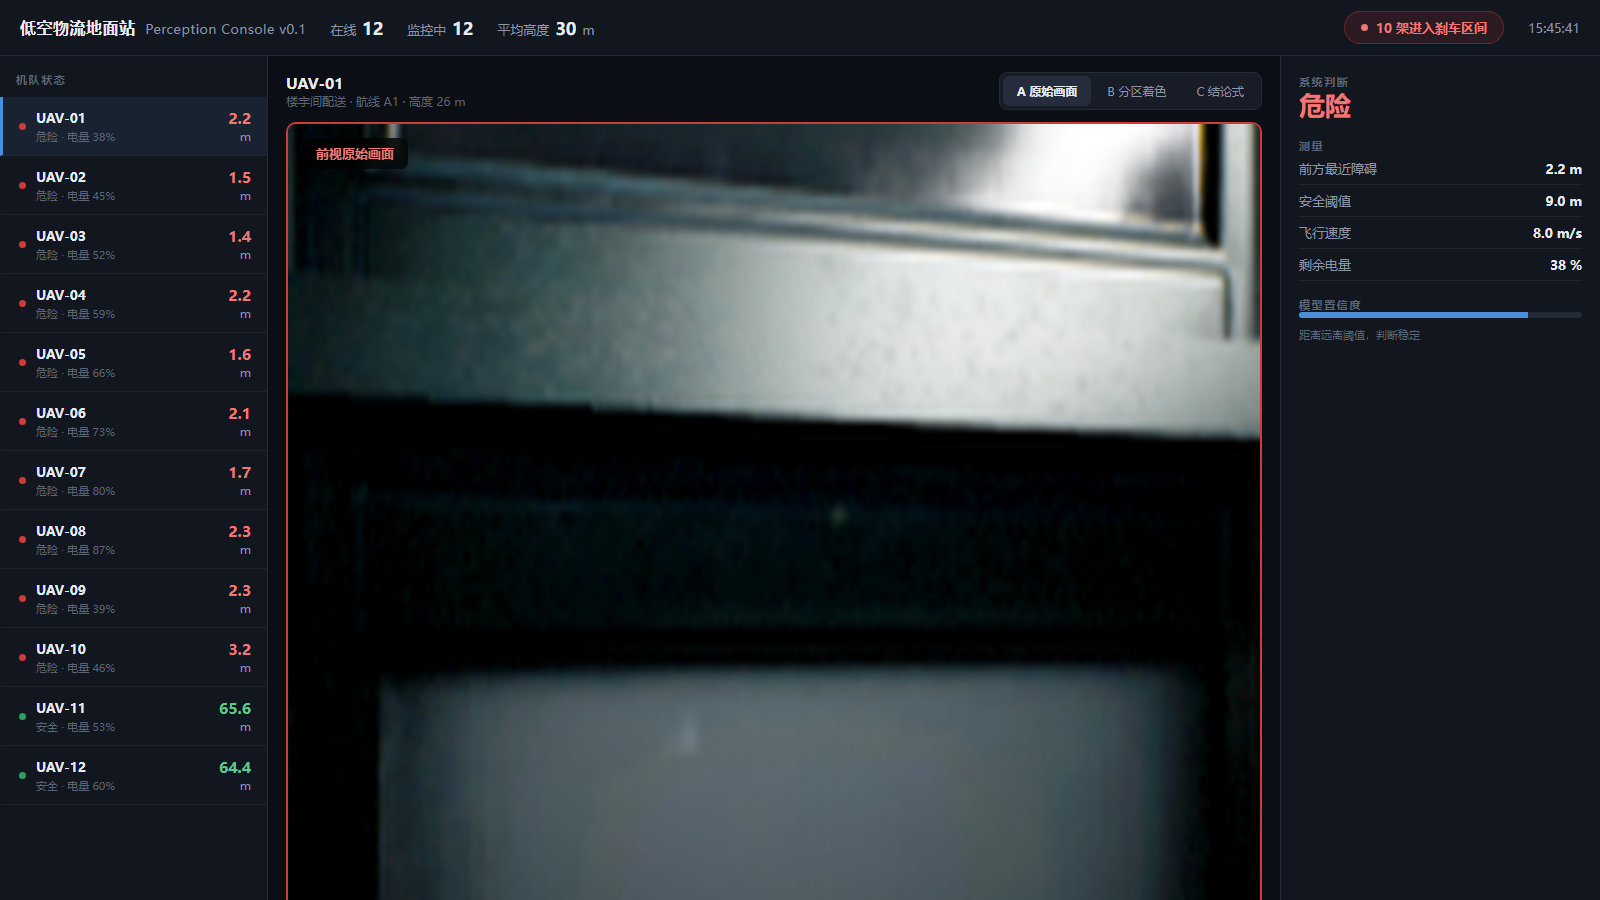
\includegraphics[width=\textwidth]{figs/console.png}
\caption{地面站原型界面。左栏为机队列表，中栏为主视图，右栏自上而下为系统判断、测量值、模型置信度与操作按钮。顶栏汇总在线数量与告警计数。}
\label{fig:console}
\end{figure}

\subsection{三种呈现模式}

中栏的主视图提供三种模式，对应三种信息密度。三版使用完全相同的画面素材与相同的判据，差别只在呈现。

\paragraph{A 版\quad 裸画面（基线）}
只显示前视画面，不给任何模型信息。这一版代表没有智能辅助时人的自然能力，作为对照基准。它的价值在于测出一个前提：人靠肉眼看单目画面，究竟能不能判断前方距离。

\paragraph{B 版\quad 分区着色}
在画面上叠加半透明色块，按距离分为三段：9 米以内红色，9 至 18 米黄色，18 米以上蓝色。右上角给出图例，底部给出最近障碍的具体数值。这一版把模型的输出翻译成空间信息，保留人自行解读的余地。它的假设是，颜色分区降低了数值比对的认知负荷，同时因为信息是空间展开的，人能看出障碍在画面中的位置。

\paragraph{C 版\quad 结论式}
画面加一圈边框，边框颜色即风险等级，顶部一行文字给出结论，底部一行给出建议动作。不给具体距离数值。这一版把模型的判断直接呈现为结论，效率最高。它的风险也最明确：当模型判断错误时，界面会以一种非常笃定的方式把错误传递给人。

三版的信息量递增，人的认知负荷递减，但对模型的依赖递增。这个此消彼长的关系是本次设计的核心张力。

\begin{figure}[htbp]
\centering
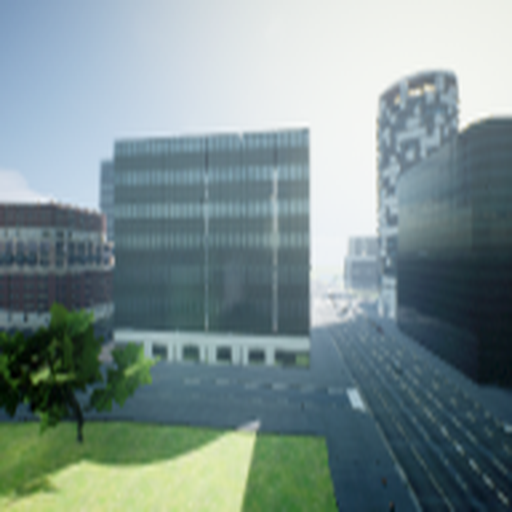
\includegraphics[width=0.32\textwidth]{stimuli/sq/f14_A.png}\hfill
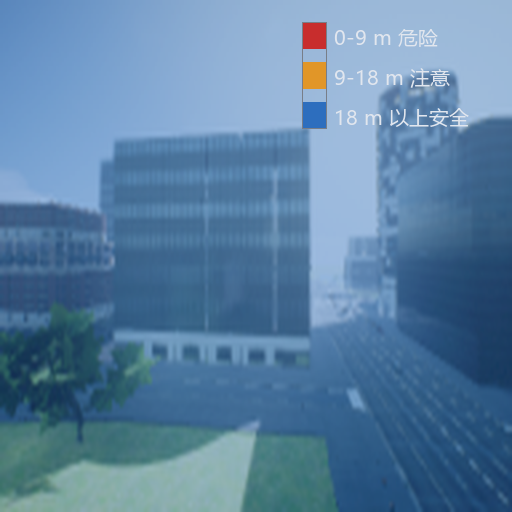
\includegraphics[width=0.32\textwidth]{stimuli/sq/f14_B.png}\hfill
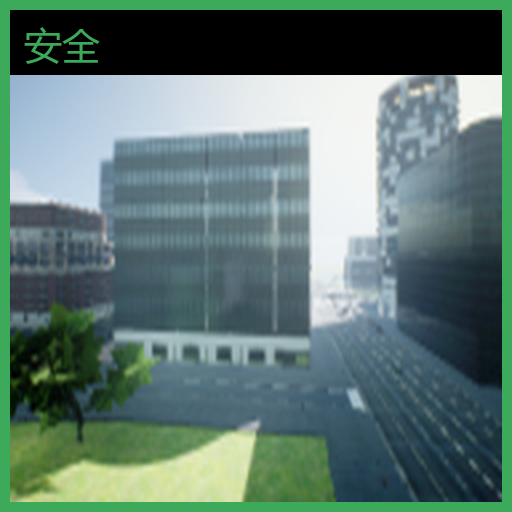
\includegraphics[width=0.32\textwidth]{stimuli/sq/f14_C.png}
\caption{同一帧画面的三种呈现模式。左为 A 版裸画面，中为 B 版分区着色，右为 C 版结论式。}
\label{fig:three}
\end{figure}

\subsection{状态与告警}

系统定义四级状态：正常、注意、危险、失联。颜色不单独承载信息，同一时刻同步改变主视图边框、列表项色标与顶栏计数三处，避免色觉障碍用户丢失关键信息。

危险状态除了变色，还会把该机顶到列表首位并触发顶栏告警计数。失联状态整行降低不透明度，文案改为信号中断，同时把可用的操作按钮减为只保留重规划，因为无画面时无法判断悬停是否安全。

\subsection{交互与操作}

点击左栏任意一架即切换主视图。顶部三个按钮切换呈现模式。右栏底部三个操作按后果严重程度自上而下排列：立即悬停用实心红底并绑定快捷键 H，减速至 3 米每秒为次要操作，重规划航线为常规操作。

\begin{table}[htbp]
\centering
\caption{三版呈现模式的信息结构与预期效果}
\label{tab:schemes}
\begin{tabular}{p{2.2cm}p{2.6cm}p{2.4cm}p{3.4cm}p{3.4cm}}
\toprule
模式 & 给出的信息 & 人的角色 & 预期优势 & 预期风险 \\
\midrule
A 裸画面 & 仅画面 & 完全自主判断 & 不受模型错误影响 & 慢，且非专业者判断力弱 \\
B 分区着色 & 画面加距离分区 & 半自主，自行解读 & 兼顾速度与独立判断 & 需要读图例，有学习成本 \\
C 结论式 & 画面加结论 & 依赖模型 & 最快最省力 & 模型错时跟随出错 \\
\bottomrule
\end{tabular}
\end{table}

\section{用户测试}

\subsection{被试与任务}

被试为在校学生，非飞行相关专业，无无人机操作经验。计划招募 10 人，采用被试内设计，每人都完成三种模式的全部试次。

情境设定为复核任务：屏幕提示某架飞机已因前方障碍自动悬停，被试看到的是那一帧的前视画面，需要判断应当解除悬停让飞机继续，还是维持悬停等待处理。

测试材料为 20 帧画面，其中 10 帧真值距离小于 9 米，属于应当维持悬停；10 帧大于 60 米，属于系统误检、应当解除。20 帧在两端刻意拉开，避免边界样本带来的噪声，先测出三种模式之间的最大差异，再在后续版本中引入边界样本。

20 帧乘以 3 种模式共 60 个试次，随机顺序呈现。被试在画面出现后尽快用键盘左右方向键作答，左为维持悬停，右为解除。程序记录选择与反应时。

\subsection{指标}

三项指标。第一是判断正确率，与真值比较，即该维持悬停时是否维持、该解除时是否解除。第二是反应时间，从画面加载完成到按键。第三是抗误导能力，在模型判断与真值不一致的子集上，统计被试跟随模型出错的比例。

第三项是本次设计最关心的指标。它直接回答一个问题：界面的笃定程度，会不会让人放弃自己的判断。

\subsection{预期与记录}

预期 C 模式在模型判断正确的帧上最快最准，在模型判断错误的帧上错误率最高。B 模式应居中。A 模式最慢，但在模型出错的帧上不受影响。

若该预期成立，设计结论是：结论式呈现适合模型置信度高的场景，分区着色适合置信度不明或人需要在环的场景，二者应当在同一套系统中按置信度切换，而不是二选一。

\begin{table}[htbp]
\centering
\caption{用户测试记录表（待填写）}
\label{tab:result}
\begin{tabular}{lccc}
\toprule
方案 & 正确率 & 平均反应时 & 模型出错帧上的跟随率 \\
\midrule
A 裸画面 & 待测 & 待测 & 待测 \\
B 分区着色 & 待测 & 待测 & 待测 \\
C 结论式 & 待测 & 待测 & 待测 \\
\bottomrule
\end{tabular}
\end{table}

\section{项目总结}

\subsection{项目亮点}

\paragraph{从算法指标转向交互后果}
项目没有停在深度估计的误差数字上，而是追问这个误差对人意味着什么。把像素误差换算成漏判与误刹，再换算成界面上的信息呈现，形成了一条从模型到人的完整链条。

\paragraph{以信息密度为唯一变量的方案设计}
三版界面使用同样的素材、同样的判据，只改变信息量这一个变量，使得测试结果可以归因于设计本身，而不是素材差异。

\paragraph{技术为设计提供参数而非结论}
深度模型的输出在本项目中不作为成果展示，而是作为设计输入。模型在哪里不可靠，决定了界面在哪里必须示弱。这个关系是本项目区别于纯算法研究的关键。

\paragraph{可复用的测试协议}
测试程序与素材以网页形式实现，被试可独立完成，数据自动记录为结构化格式，便于扩大样本与重复实验。

\subsection{项目经验}

\paragraph{设计问题往往藏在技术指标的背面}
如果只看 $\delta_1$ 是 0.858，会认为模型已经可用。但把剩下的 14\% 展开，看到的是漏判集中在玻璃幕墙与远距离结构上，这才构成了真实的设计约束。指标的背面是失效模式，失效模式才是设计的起点。

\paragraph{信任是需要设计的，不能默认}
自动驾驶领域的经验说明，人对自动化系统的信任既可能不足也可能过度。界面越是把结论说得笃定，人越容易放弃复核。这一点在只有几秒决策窗口的无人机场景下后果更严重。

\paragraph{原型要早做，测试要早跑}
界面方案的价值只有在被试手上才能验证。逻辑上再合理的配色与布局，都可能在实际使用中被误解。本项目把原型与测试协议提前到方案定稿之前完成，为迭代留出时间。

\section{结语}

低空物流的规模化，最终卡在信任上。不是人信不过机器，而是机器从不告诉人它有多确信。本文做的工作很有限，只是把这一层缺失具体化成三版界面、二十帧素材和一套测试协议。但它指向的问题很实在：当智能系统接管了判断，界面就不该只是结果的显示器，它应该是系统状态与人之间的翻译。

\section*{项目分工}
\addcontentsline{toc}{section}{项目分工}

（待填写，按实际参与者补全）

\begin{thebibliography}{9}
\addcontentsline{toc}{section}{参考文献}

\bibitem{bainbridge} Bainbridge L. Ironies of Automation[J]. Automatica, 1983, 19(6): 775-779.

\bibitem{parasuraman} Parasuraman R, Riley V. Humans and Automation: Use, Misuse, Disuse, Abuse[J]. Human Factors, 1997, 39(2): 230-253.

\bibitem{endsley} Endsley M R, Kiris E O. The Out-of-the-Loop Performance Problem and Level of Control in Automation[J]. Human Factors, 1995, 37(2): 381-394.

\bibitem{midas} Ranftl R, Lasinger K, Hafner D, et al. Towards Robust Monocular Depth Estimation: Mixing Datasets for Zero-shot Cross-dataset Transfer[J]. IEEE Transactions on Pattern Analysis and Machine Intelligence, 2022, 44(3): 1623-1637.

\bibitem{da} Yang L, Kang B, Huang Z, et al. Depth Anything: Unleashing the Power of Large-Scale Unlabeled Data[C]. IEEE/CVF Conference on Computer Vision and Pattern Recognition, 2024.

\bibitem{monodepth2} Godard C, Mac Aodha O, Firman M, et al. Digging Into Self-Supervised Monocular Depth Estimation[C]. IEEE/CVF International Conference on Computer Vision, 2019.

\bibitem{resnet} He K, Zhang X, Ren S, et al. Deep Residual Learning for Image Recognition[C]. IEEE Conference on Computer Vision and Pattern Recognition, 2016.

\bibitem{vjepa} Mur-Labadia L, Muckley M, Bar A, et al. V-JEPA 2.1: Unlocking Dense Features in Video Self-Supervised Learning[J]. arXiv preprint arXiv:2603.14482, 2026.

\end{thebibliography}

\end{document}
